\documentclass[twoside]{article}
\usepackage{algorithm}
\usepackage{algorithmic}
\usepackage{amssymb,amsmath,amsthm}
\usepackage{graphicx}
\usepackage{preamble}
\usepackage{natbib}
\usepackage{hyperref}
\usepackage{color}
\usepackage{wasysym}
\usepackage{subfigure}
\usepackage{tabularx}
\usepackage{bm}
\newcommand{\theHalgorithm}{\arabic{algorithm}}
\definecolor{mydarkblue}{rgb}{0,0.08,0.45}
\hypersetup{ %
    pdftitle={},
    pdfauthor={},
    pdfsubject={},
    pdfkeywords={},
    pdfborder=0 0 0,
    pdfpagemode=UseNone,
    colorlinks=true,
    linkcolor=mydarkblue,
    citecolor=mydarkblue,
    filecolor=mydarkblue,
    urlcolor=mydarkblue,
    pdfview=FitH}

\newcolumntype{x}[1]{>{\centering\arraybackslash\hspace{0pt}}m{#1}}
\newcommand{\tabbox}[1]{#1}
    
%%%%%%%%%%%%%%%%%%%%%%%%%%%%%%%%%%%%%%%%%%%%%%%%%%%%%%%%%%
%%%% EDITING HELPER FUNCTIONS  %%%%%%%%%%%%%%%%%%%%%%%%%%%
%%%%%%%%%%%%%%%%%%%%%%%%%%%%%%%%%%%%%%%%%%%%%%%%%%%%%%%%%%

%% NA: needs attention (rough writing whose correctness needs to be verified)
%% TBD: instructions for how to fix a gap ("Describe the propagation by ...")
%% PROBLEM: bug or missing crucial bit 

%% use \fXXX versions of these macros to put additional explanation into a footnote.  
%% The idea is that we don't want to interrupt the flow of the paper or make it 
%% impossible to read because there are a bunch of comments.

%% NA's (and TBDs, those less crucially) should be written so 
%% that they flow with the text.

\definecolor{WowColor}{rgb}{.75,0,.75}
\definecolor{SubtleColor}{rgb}{0,0,.50}

% inline
\newcommand{\NA}[1]{\textcolor{SubtleColor}{ {\tiny \bf ($\star$)} #1}}
\newcommand{\LATER}[1]{\textcolor{SubtleColor}{ {\tiny \bf ($\dagger$)} #1}}
\newcommand{\TBD}[1]{\textcolor{SubtleColor}{ {\tiny \bf (!)} #1}}
\newcommand{\PROBLEM}[1]{\textcolor{WowColor}{ {\bf (!!)} {\bf #1}}}

% as margin notes

\newcounter{margincounter}
\newcommand{\displaycounter}{{\arabic{margincounter}}}
\newcommand{\incdisplaycounter}{{\stepcounter{margincounter}\arabic{margincounter}}}

\newcommand{\fTBD}[1]{\textcolor{SubtleColor}{$\,^{(\incdisplaycounter)}$}\marginpar{\tiny\textcolor{SubtleColor}{ {\tiny $(\displaycounter)$} #1}}}

\newcommand{\fPROBLEM}[1]{\textcolor{WowColor}{$\,^{((\incdisplaycounter))}$}\marginpar{\tiny\textcolor{WowColor}{ {\bf $\mathbf{((\displaycounter))}$} {\bf #1}}}}

\newcommand{\fLATER}[1]{\textcolor{SubtleColor}{$\,^{(\incdisplaycounter\dagger)}$}\marginpar{\tiny\textcolor{SubtleColor}{ {\tiny $(\displaycounter\dagger)$} #1}}}

\usepackage{format/icml2013}

%% For submission, make all render blank.
%\renewcommand{\LATER}[1]{}
%\renewcommand{\fLATER}[1]{}
%\renewcommand{\TBD}[1]{}
%\renewcommand{\fTBD}[1]{}
%\renewcommand{\PROBLEM}[1]{}
%\renewcommand{\fPROBLEM}[1]{}
%\renewcommand{\NA}[1]{#1}  %% Note, NA's pass through!
    
%\subsection{How to use commenting}
%\NA{Needs attention.}
%\TBD{To be done.}
%\PROBLEM{Problem.}
%\fTBD{Margin to be done.}
%\fPROBLEM{Margin problem.}
    
\begin{document}

\twocolumn[
\icmltitle{Kernel Structure Discovery}
%\icmlauthor{Anonymous Authors}
%\icmladdress{ Unknown Institution}
\icmlkeywords{nonparametrics, gaussian process, machine learning, ICML}
\vskip 0.3in
]


\begin{abstract}
%\TBD{Shift focus away from GPs?}
Gaussian process (GP) models are used widely and successfully.
However, their effictiveness depends critically on choosing an appropriate family of kernels.
This aspect of GP modeling has been sorely underdeveloped.
In this paper, we introduce a procedure for automatically and efficiently searching through a large space of GP models.
\end{abstract}

\section{Introduction}

Similar searches over large model classes have been succesfully used in machine vision [cite Cox + Pinto].
In general, learning the model class from data seems superior proposing the model beforehand.
In high dimensional problems, it is also hard for a practitioner to propose an appropriate model even after examining a dataset closely.
Choosing a kernel family is also a stumbling block for non-experts who wish to use Gaussian Process models.

[Zoubin says: There has been tons of work done on automatic structure discovery in unsupervised settings, but little done in supervised learning.]

\section{Gaussian Processes Priors}

Gaussian processes are a flexible and tractable prior over functions, useful for solving regression and classification tasks\cite{rasmussen38gaussian}.
The kind of structure which can be captured by a GP model is mainly determined by its \emph{kernel}: the covariance function.
One of the main difficulties in specifying a Gaussian process model is in choosing a kernel which can represent the structure present in the data.
For small to medium-sized datasets, the kernel has a large impact on modeling efficacy.

\TBD{Note: The above paragraph is plagarized from my additive GP paper. -David} 

[TODO: add GP math intro\TBD{ Really? Just cite?}]

\section{Expressing Structure through Kernels}

[Emphasize that these techniques could work on SVMs, but that this would be difficult because model selection is hard without evidence measures]

[Explain exactly how one can express structure on functions, with examples]

Examples: Local linear structure, local periodicity.

Figure \ref{fig:kernels} shows how to construct such structures as:  Long-range trends with local variation, local periodicity, long-range trends 

\newcommand{\fwb}{2.45cm}  % width
\newcommand{\fwh}{1.6cm}     % height
\begin{figure}[t]
\centering
\begin{tabular}{C{\fwb}C{\fwb}C{\fwb}}
%kernel & draws from GP & GP posterior \\
\rotatebox{90}{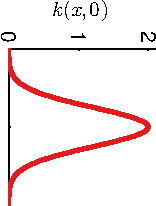
\includegraphics[width=\fwh,height=\fwb]{../figures/structure_examples/se_kernel}} &  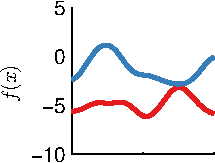
\includegraphics[width=\fwb,height=\fwh]{../figures/structure_examples/se_kernel_draws} & 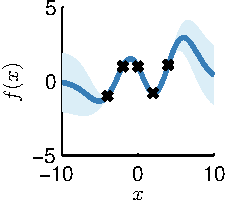
\includegraphics[width=\fwb,height=\fwh]{../figures/structure_examples/se_kernel_post} \\
squared-exp & \multicolumn{2}{c}{locally smooth} \\ \midrule
\rotatebox{90}{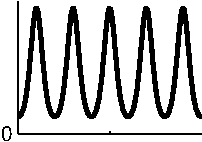
\includegraphics[width=\fwh,height=\fwb]{../figures/structure_examples/per_kernel}} &  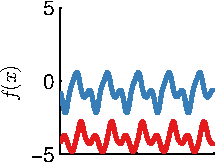
\includegraphics[width=\fwb,height=\fwh]{../figures/structure_examples/per_kernel_draws} & 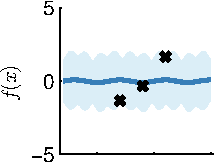
\includegraphics[width=\fwb,height=\fwh]{../figures/structure_examples/per_kernel_post} \\
periodic & \multicolumn{2}{c}{repeated structure} \\ \midrule
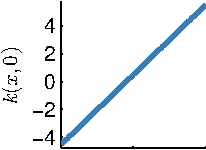
\includegraphics[width=\fwb,height=\fwh]{../figures/structure_examples/lin_kernel} &  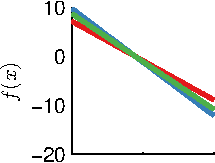
\includegraphics[width=\fwb,height=\fwh]{../figures/structure_examples/lin_kernel_draws} & 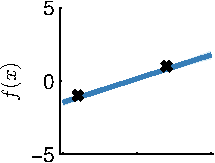
\includegraphics[width=\fwb,height=\fwh]{../figures/structure_examples/lin_kernel_post} \\
linear & \multicolumn{2}{c}{linear functions} \\ \midrule
\rotatebox{90}{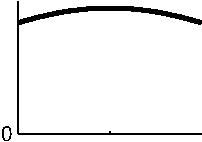
\includegraphics[width=\fwh,height=\fwb]{../figures/structure_examples/longse_kernel}} &  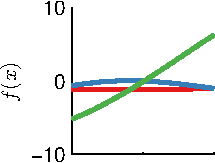
\includegraphics[width=\fwb,height=\fwh]{../figures/structure_examples/longse_kernel_draws} & 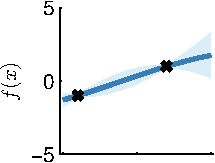
\includegraphics[width=\fwb,height=\fwh]{../figures/structure_examples/longse_kernel_post} \\
long-length SE & \multicolumn{2}{c}{slowly changing}
\end{tabular}
\caption{ Properties of basic kernels.  Left: base kernels. Centre:  draws from a \gp{} with that kernel.  Right: a GP posterior after conditioning on three datapoints.
\TBD{RBG: Do we need this figure?  It's pretty standard stuff, and it's largely subsumed by Figure 2.}}
\label{fig:basic_kernels}
\end{figure}


\newcommand{\fw}{2.6cm}
\begin{figure*}
\centering
\begin{tabular}{ccccc|c|c}
& & & & 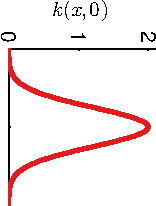
\includegraphics[width=\fw]{../figures/structure_examples/se_kernel} &  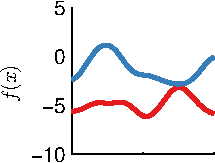
\includegraphics[width=\fw]{../figures/structure_examples/se_kernel_draws} & 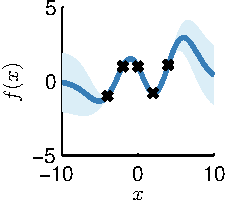
\includegraphics[width=\fw]{../figures/structure_examples/se_kernel_post} \\
& & & & 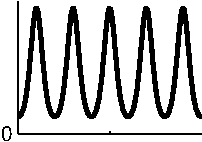
\includegraphics[width=\fw]{../figures/structure_examples/per_kernel} &  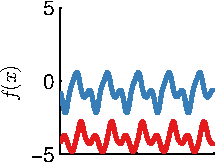
\includegraphics[width=\fw]{../figures/structure_examples/per_kernel_draws} & 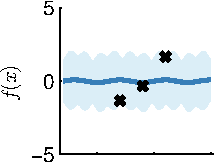
\includegraphics[width=\fw]{../figures/structure_examples/per_kernel_post} \\
& & & & 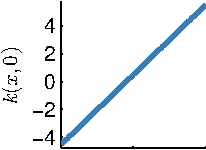
\includegraphics[width=\fw]{../figures/structure_examples/lin_kernel} &  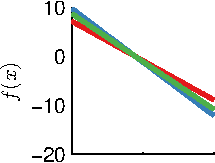
\includegraphics[width=\fw]{../figures/structure_examples/lin_kernel_draws} & 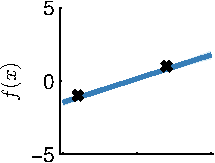
\includegraphics[width=\fw]{../figures/structure_examples/lin_kernel_post} \\
 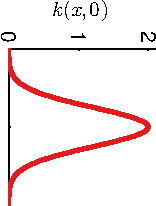
\includegraphics[width=\fw]{../figures/structure_examples/se_kernel} & $\times$ & 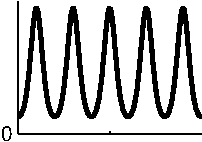
\includegraphics[width=\fw]{../figures/structure_examples/per_kernel} & = & 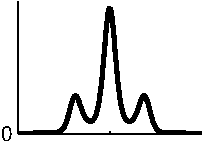
\includegraphics[width=\fw]{../figures/structure_examples/se_times_per} & 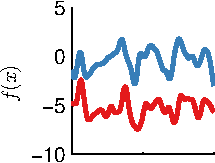
\includegraphics[width=\fw]{../figures/structure_examples/se_times_per_draws} & 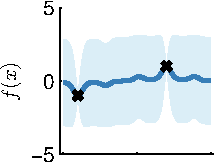
\includegraphics[width=\fw]{../figures/structure_examples/se_times_per_post} \\
  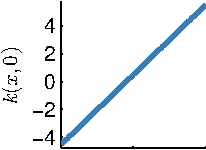
\includegraphics[width=\fw]{../figures/structure_examples/lin_kernel} & $\times$ & 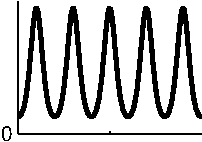
\includegraphics[width=\fw]{../figures/structure_examples/per_kernel} & = & 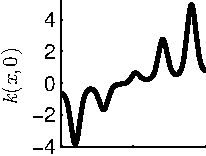
\includegraphics[width=\fw]{../figures/structure_examples/lin_times_per} & 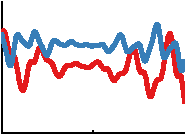
\includegraphics[width=\fw]{../figures/structure_examples/lin_times_per_draws} & 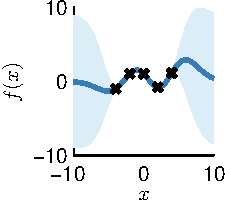
\includegraphics[width=\fw]{../figures/structure_examples/se_times_lin_post} \\
   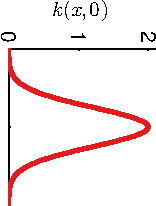
\includegraphics[width=\fw]{../figures/structure_examples/se_kernel} & $+$ & 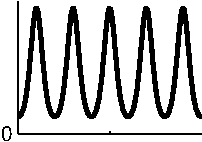
\includegraphics[width=\fw]{../figures/structure_examples/per_kernel} & = & 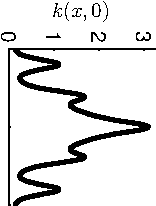
\includegraphics[width=\fw]{../figures/structure_examples/se_plus_per} & 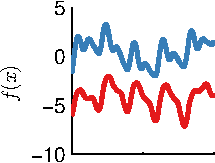
\includegraphics[width=\fw]{../figures/structure_examples/se_plus_per_draws} & 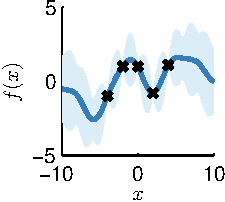
\includegraphics[width=\fw]{../figures/structure_examples/se_plus_per_post} \\
  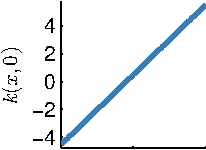
\includegraphics[width=\fw]{../figures/structure_examples/lin_kernel} & $+$ & 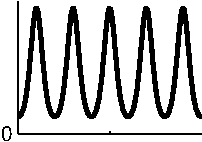
\includegraphics[width=\fw]{../figures/structure_examples/per_kernel} & = & 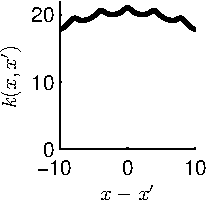
\includegraphics[width=\fw]{../figures/structure_examples/lin_plus_per} & 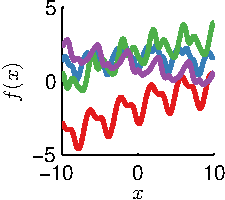
\includegraphics[width=\fw]{../figures/structure_examples/lin_plus_per_draws} & 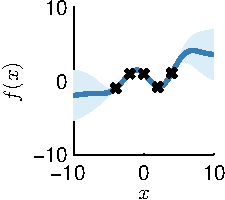
\includegraphics[width=\fw]{../figures/structure_examples/se_plus_lin_post} \\
   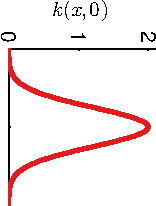
\includegraphics[width=\fw]{../figures/structure_examples/se_kernel} & $+$ & 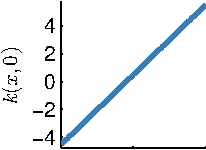
\includegraphics[width=\fw]{../figures/structure_examples/lin_kernel} & = & 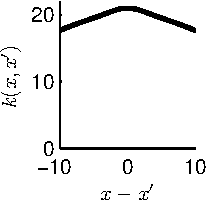
\includegraphics[width=\fw]{../figures/structure_examples/se_plus_lin} & 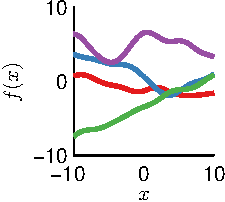
\includegraphics[width=\fw]{../figures/structure_examples/se_plus_lin_draws} & 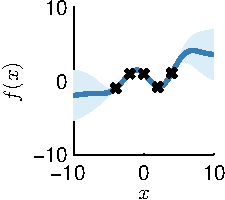
\includegraphics[width=\fw]{../figures/structure_examples/se_plus_lin_post} \\
   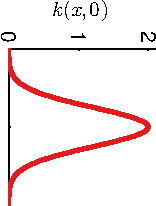
\includegraphics[width=\fw]{../figures/structure_examples/se_kernel} & $\times$ & 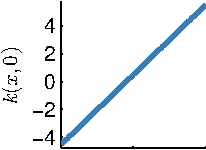
\includegraphics[width=\fw]{../figures/structure_examples/lin_kernel} & = & 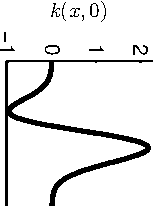
\includegraphics[width=\fw]{../figures/structure_examples/se_times_lin} & 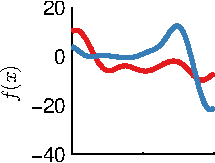
\includegraphics[width=\fw]{../figures/structure_examples/se_times_lin_draws} & \includegraphics[width=\fw]{../figures/structure_examples/se_times_lin_post} \\
base kernel & & base kernel & & combined kernel & draws from GP & GP posterior
\end{tabular}
\caption{ A draw from a sum of kernels corresponds to a sum of draws from the base kernels.  A draw from a product kernel prior has weaker long-range dependencies, and less long-range structure.
}
\label{fig:kernels}
\end{figure*}

\subsection{Convenience Priors}

One of the main advantage of kernel methods, and Gaussian process regression in particular, is that the kernel can be used to specify interesting prior structure to the model.
However, in practice, GPs are typically used with only the squared-exp kernel.
[Apparently, this was one of Sholkopf's big dissapointment with GPs... is there a quote from him on this? -David]

A frequent criticism of the Bayesian framework is that priors are often chosen purely for convenience.  Gaussian process priors may be a good examples of a model chosen for its tractability.
However, specifying a compound kernel typically does not change the order of computational complexity of inference in Gaussian process models.
The broad use of simple kernels may be simply due to the difficulty of determining which kinds of structure exist in the data and guessing how to express that through a covariance function.
Hence, automating the search over kernel structures should be especially useful in allowing pracitioners from a wide variety of backgrounds to use appropriate models for their data.
Indeed, the authors of this paper were sometimes surprised by the kernels chosen by the automated search, which were able to express structure which was not obvioulsy expressible through a simple combination of kernels.

\subsection{Decomposing the Signal}

The sorts of structure implied by complex kernel might not be immediately interpretable.
However, there is one property of GPs that allows us to break down the signal into interpretable parts.
Specifically, a function $f \sim GP(0, k_1(x, x') + k_2(x,x')$, whose kernel is a sum of kernels, has the same distribution as a sum of two functions $\vf = \vf_1 + \vf_2$ where $\vf_1 \sim \gp( \vmu_1, k_1)$ and $\vf_2 \sim \gp( \vmu_2, k_2)$.
In addition, the posterior distributions over individual components after conditioning on data are also analytically tractable.

The conditional distribution of a Gaussian $\vf_1$ conditioned on its sum with another Gaussian $\vf = \vf_1 + \vf_2$ where $\vf_1 \sim \gp( \vmu_1, k_1)$ and $\vf_2 \sim \gp( \vmu_2, k_2)$ is given by
\begin{align}
\vf_1^\star | \vf \sim \mathcal{N} \big( & \vmu_1^\star + \vk_1^\star (\vK_1 + \vK_2)\inv \left( \vf - \vmu_1 - \vmu_2 \right), \nonumber \\
& \vk_1^{\star\star} - \vk_1^\star (\vK_1 + \vK_2)\inv \vk_1^\star \big).
\end{align}
and the covariance between the two components, conditioned on their sum is given by:
\begin{align}
\cov(\vf_1^\star, \vf_2^\star) | \vf = \vk_1^{\star\tra} (\vK_1 + \vK_2)\inv \vk_2^\star
\end{align}
Derivations are in the supplementary material.

These distributions express the posterior model uncertainty about different components of the signal, integrating over the possible configurations of the other components.
These expressions allow us to decompose the posterior into a sum of interpretable parts, and examine each one in turn.

\TBD{Check that the notation for stars and kernel matrices is explained somewhere.}
\TBD{Smooth the flow of the previous subsection.}

\section{Searching over structures}

\TBD{Needs works e.g.~justification / cite Roger and other grammar based search papers. Is there a canonical paper for forward variable selection in linear models?}

Notes on the algorithm
\begin{enumerate}
\item Initial set of kernels $\mathcal{K}$ = all base kernels $\times$ applied to all single input dimensions $\times$ random kernel parameter initialisations
\item For each $\kappa \in \mathcal{K}$ optimise parameters by optimising nll on training data; record nll and BIC
\item Remove approximately duplicate `kernels' by standardising forms, detecting equivalent parameters and examining Frobenius norm between covariance matrices (\TBD{this heuristic to be examined - currently not used in results presented since $k = 1$ - see below}).
\item Set $\mathcal{K}^*$ = best $k$ kernels as determined by BIC
\item Set $\mathcal{K}$ = expansion of all kernels in $\mathcal{K}^*$ with some random initialisations of new kernel parameters (keeping previously learned parameters - practically this is quite important)
\item Return to step 2, repeating until some fixed depth $D$ (\TBD{this could be replaced with stopping when no kernel is an improvement})
\end{enumerate}

Expanding a kernel involves
\begin{itemize}
\item For each kernel component (i.e.~any product, sum or base kernel)
\item Either add by, multiply by or replace with (only base kernels) all base kernels $\times$ applied to all single input dimensions
\item \TBD{Experiments suggest that pruning `expansions' may be beneficial when the base kernel space is large - not yet implemented}
\end{itemize}

\section{Related Work}

Compositional Model search for unsupervsied learning: \cite{grosse2012exploiting}

Hyperkernels \cite{ong2002hyperkernels}

\paragraph{ANOVA Kernels}

Support vector regression with ANOVA decomposition kernels \cite{stitson1999support}

%\subsubsection{Smoothing spline ANOVA models}
A closely related procedure from the statistics literature is smoothing-splines ANOVA (SS-ANOVA)\cite{wahba1990spline, gu2002smoothing}.
An SS-ANOVA model is estimated as a weighted sum of splines along each dimension, plus a sum of splines over all pairs of dimensions, all triplets, etc, with each individual interaction term having a separate weighting parameter.
Because the number of terms to consider grows exponentially in the order, in practice, only terms of first and second order are usually considered.  Learning in SS-ANOVA is usually done via penalized-maximum likelihood with a fixed sparsity hyperparameter.

\paragraph{Hierarchical Kernel Learning}

In "High-Dimensional Non-Linear Variable Selection through Hierarchical Kernel Learning", Bach\cite{DBLP:journals/corr/abs-0909-0844} uses a regularized optimization framework to learn a weighted sum over an exponential number of kernels which can be computed in polynomial time.
The subsets of kernels considered by this method are restricted to be a \textit{hull} of kernels.\footnote{In the setting we are considering in this paper, a hull can be defined as a subset of all terms such that if term $\prod_{j \in J} k_j(\bf x, x')$ is included in the subset, then so are all terms $\prod_{j \in J / i} k_j(\bf x, x')$, for all $i \in J$.
For details, see \cite{DBLP:journals/corr/abs-0909-0844}.}
Given each dimension's kernel, and a pre-defined weighting over all terms, HKL performs model selection by searching over hulls of interaction terms.
% \subsubsection{All-subsets kernel with uniform weightings}
In \cite{DBLP:journals/corr/abs-0909-0844}, Bach also fixes the relative weighting between orders of interaction with a single term $\alpha$, computing the sum over all orders by:
\begin{equation}
\label{eqn:uniform}
k_{a}({\bf x, x'}) = v_D^2 \prod_{d=1}^D \left(1 + \alpha k_{d}(x_{d}, x_{d}') \right)
\end{equation}
which has computational complexity $O(D)$.
However, this formulation forces the weight of all $n$th order terms to be weighted by $\alpha^n$.

The main difficulty with the approach of \cite{DBLP:journals/corr/abs-0909-0844} is that hyperparameters are hard to set other than by cross-validation. 
In contrast, our method optimizes the hyperparameters of each dimension's base kernel, as well as the relative weighting of each order of interaction. 

Accuracy versus interpretability in flexible modeling: Implementing a tradeoff using Gaussian process models \cite{plate1999accuracy}

A related functional ANOVA GP model\cite{kaufman2010bayesian} decomposes the \emph{mean} function into a weighted sum of GPs.
However, the effect of a particular degree of interaction cannot be quantified by that approach.
Also, computationally, the Gibbs sampling approach used in \cite{kaufman2010bayesian} is disadvantageous.

\paragraph{Genetic Searches}

Evolving kernel functions for SVMs by genetic programming: \cite{diosan2007evolving}

A Genetic Programming based kernel construction and optimization method for Relevance Vector Machines: \cite{bing2010gp}

\paragraph{Equation Learning}

Equation discovery with ecological applications \cite{dzeroski1999equation}

Discovering admissible model equations from observed data based on scale-types and identity constraints \cite{washio1999discovering}

\paragraph{Multiple Kernel Learning}

\cite{christoudias2009bayesian} previously showed how mixtures of kernels can be learnt by gradient descent in the Gaussian process framework.
They call this \emph{Bayesian localized multiple kernel learning}.

\paragraph{Using DBNs to learn a kernel function}

\TBD{Cite relevant work by Salkhutdinov and Hinton}

\section{Experiments}

To evaluate the effectiveness of our method we performed two types of experiments; testing the ability of the algorithm to infer both an accurate regression function estimate and to produce an interpretable decomposition of a regression function.
The accuracy experiments show that our method consistently matches or beats previous state of the art regression methods (\TBD{not yet statistically significantly within each experiment - more experiments currently running\ldots}).
The decomposition experiments produce highly interpretable decompositions of time series data and highly plausible extrapolations; a particularly rare property of naively applied (linear) smoothers (\TBD{justify comment - e.g.~local linear is just linear, GP Sq-Exp nose dives towards the mean}).

\subsection{Decomposition}

We demonstrate the decompositions produced by our method on two time series.
For the search we used $k = 1$, $D = 8$ and four base kernels; SE, PE, RQ and LN (see table~\ref{tbl:kernel_descriptions}) \TBD{these were chosen to minimally (without parameter degeneracy e.g.~RQ could approximate SE and LN) allow the discovery of smooth functions, smooth periodic functions, rough functions and linear structure}.

%% --- Automatically generated by latex.py ---
% Exported at 2013-01-28 17:50:37.602844
\begin{table}[h!]
\begin{center}
\begin{tabular}{l | l l l}
   & \rotatebox{0}{ Description }  & \rotatebox{0}{ Parameters }  \\ \hline
SE & Squared-exponential  & lengthscale  \\
RQ & Rational Quadratic  & lengthscale, alpha  \\
LN & Linear  & none  \\
P & Piecewise Polynomial 1  & lengthscale  \\
MT & Mat\'{e}rn  & lengthscale  \\
\end{tabular}
\end{center}
\label{tbl:kernel_descriptions}
\end{table}


\paragraph{Mauna Loa Atmospheric Carbon Dioxide}

As an example of a GP modeling problem where choosing an appropriate structure is critical, we revisit a dataset explored in \cite{rasmussen38gaussian}, pages 120-126, where a kernel was hand-tailored to fit a GP model to the dataset.

Figures \ref{fig:mauna_grow} show the posterior's increasingly appropriate model as the search depth increases on the Mauna Loa dataset.
Note in particular that whilst the interior of the data can be smoothed effectively with a single base kernel model, the extrapolations improve dramatically as the search descends.

Figure \ref{fig:mauna_decomp} shows the complete posterior of the maximum depth $\gp$ regression model together with the additive components of the posterior.
The plot shows a very plausible extrapolation and highly interpretable components i.e.~a long-term trend, annual periodicity, medium-term deviations and short-term serially correlated `noise'.

\begin{figure}[h!]
\centering
\newcommand{\wmg}{8cm}  % width maunu growth
\newcommand{\hmg}{4cm}  % height maunu growth
\begin{tabular}{c}
 \includegraphics[width=\wmg,height=\hmg]{../figures/decomposition/03-mauna2003_max_level_0/03-mauna2003_all} \\ 
 \includegraphics[width=\wmg,height=\hmg]{../figures/decomposition/03-mauna2003_max_level_1/03-mauna2003_all} \\
 \includegraphics[width=\wmg,height=\hmg]{../figures/decomposition/03-mauna2003_max_level_2/03-mauna2003_all}
\end{tabular}
\caption{Posterior mean and variance for different depths of kernel search.  In the first row, the function is only modeled as a locally smooth function, and the extrapolation is extemely poor.  In the second, a periodic component is added, and the extrapolation is better.  At depth 3, the kernel can capture most of the relevant structure, and is able to extrapolate reasonably.}
\label{fig:mauna_grow}
\end{figure}

\begin{figure}[h!]
\newcommand{\wmgd}{8cm}  % width mauna growth decomp
\newcommand{\hmgd}{3cm}  % height mauna growth decomp
\begin{tabular}{c}
 \includegraphics[width=\wmgd,height=\hmgd]{../figures/decomposition/03-mauna2003_max_level_8/03-mauna2003_all} \\ = \\
 \includegraphics[width=\wmgd,height=\hmgd]{../figures/decomposition/03-mauna2003_max_level_8/03-mauna2003_3} \\ + \\
 \includegraphics[width=\wmgd,height=\hmgd]{../figures/decomposition/03-mauna2003_max_level_8/03-mauna2003_4_zoom} \\ + \\
 \includegraphics[width=\wmgd,height=\hmgd]{../figures/decomposition/03-mauna2003_max_level_8/03-mauna2003_1} \\ + \\
 \includegraphics[width=\wmgd,height=\hmgd]{../figures/decomposition/03-mauna2003_max_level_8/03-mauna2003_2} \\
\end{tabular}
\caption{First row: The posterior on the Mauna Loa dataset after a search of depth 8.  Subsequent rows: automatic decomposition of Mauna Loa data.  The signal has been automatically decomposed into long-term, yearly periodic, medium-term anomaly and short-term noise components, respectively.}
\end{figure}
\label{fig:mauna_decomp}

\paragraph{Airline passenger data}

Figures \ref{fig:airline_grow} and \ref{fig:airline_decomp} show the corresponding plots for the airline data set (\TBD{describe me!}).
\TBD{Make similar observations of good performance and perhaps draw attention to the selection of a linear kernel}.

\begin{figure}[h!]
\centering
\newcommand{\wag}{8cm}  % width airline growth
\newcommand{\hag}{4cm}  % height airline growth
\begin{tabular}{c}
 \includegraphics[width=\wag,height=\hag]{../figures/decomposition/01-airline-months_max_level_0/01-airline-months_all} \\ 
 \includegraphics[width=\wag,height=\hag]{../figures/decomposition/01-airline-months_max_level_1/01-airline-months_all} \\
 \includegraphics[width=\wag,height=\hag]{../figures/decomposition/01-airline-months_max_level_2/01-airline-months_all} \\
 \includegraphics[width=\wag,height=\hag]{../figures/decomposition/01-airline-months_max_level_3/01-airline-months_all}
\end{tabular}
\caption{Posterior mean and variance for different levels of kernel search on the airline dataset.}
\label{fig:airline_grow}
\end{figure}


\begin{figure}[h!]
\centering
\newcommand{\wagd}{8cm}  % width airline growth decomp
\newcommand{\hagd}{4cm}  % height airline growth decomp
\begin{tabular}{c}
 \includegraphics[width=\wagd,height=\hagd]{../figures/decomposition/01-airline-months_max_level_8/01-airline-months_all} \\ 
 = \\ 
 \includegraphics[width=\wagd,height=\hagd]{../figures/decomposition/01-airline-months_max_level_8/01-airline-months_1} \\
 + \\
 \includegraphics[width=\wagd,height=\hagd]{../figures/decomposition/01-airline-months_max_level_8/01-airline-months_2} \\
 + \\
 \includegraphics[width=\wagd,height=\hagd]{../figures/decomposition/01-airline-months_max_level_8/01-airline-months_3}
\end{tabular}
\caption{First row:  The airline dataset and posterior after a search of depth 8.  Rows 2-4: Additive decomposition of posterior into long-term smooth trend, yearly variation, and short-term noise.  Note that the variance of the noise grows over time, making this a heteroskedastic model.}
\label{fig:airline_decomp}
\end{figure}

\subsection{Regression accuracy}

$k = 1$, $D = 8$, kernels are SE and RQ (\TBD{currently running other experiments that may be more canonical}).

We have extended the comparison of \cite{duvenaud2011additive11} to include our method.
5 data sets were split into 10 equally sized folds.
For each fold of each data set we trained each method on the other 9 folds, and then computed predictive mean squared error (MSE) and mean negative predictive log likelihood on the held out fold (data missing at random \TBD{we could likely do much better by creating folds that remove continuous regions if extrapolation ability carries over to high dimensional data}.
Average statistics for these experiments are presented in tables \ref{tbl:Regression Mean Squared Error} and \ref{tbl:Regression Negative Log Likelihood}.

% --- Automatically generated by resultsToLatex2.m ---
% Exported at 28-Jan-2013 15:53:45
\begin{table*}[ht!]
\caption{{\small
Regression Mean Squared Error
}}
\label{tbl:Regression Mean Squared Error}
\begin{center}
\begin{tabular}{l | r r r r r}
Method & \rotatebox{0}{ bach  }  & \rotatebox{0}{ concrete  }  & \rotatebox{0}{ puma }  & \rotatebox{0}{ servo }  & \rotatebox{0}{ housing }  \\ \hline
Linear Regression & $1.031$ & $0.404$ & $0.641$ & $0.523$ & $0.289$ \\
GP GAM & $1.259$ & $0.149$ & $0.598$ & $0.281$ & $0.161$ \\
HKL & $\mathbf{0.199}$ & $0.147$ & $0.346$ & $0.199$ & $0.151$ \\
GP Squared-exp & $\mathbf{0.045}$ & $0.157$ & $0.317$ & $0.126$ & $\mathbf{0.092}$ \\
GP Additive & $\mathbf{0.045}$ & $\mathbf{0.089}$ & $\mathbf{0.316}$ & $\mathbf{0.110}$ & $0.102$ \\
%22-Jan & $\mathbf{0.513}$ & $\mathbf{0.089}$ & $\mathbf{0.312}$ & $\mathbf{0.095}$ & $\mathbf{0.091}$ \\
\hline
Structure Search & $\mathbf{0.044}$ & $\mathbf{0.087}$ & $\mathbf{0.315}$ & $\mathbf{0.102}$ & $\mathbf{0.082}$
\end{tabular}
\end{center}
\end{table*}
% End automatically generated LaTeX

% --- Automatically generated by resultsToLatex2.m ---
% Exported at 28-Jan-2013 15:53:45
\begin{table}[h!]
\caption{{\small
Regression Negative Log Likelihood
}}
\label{tbl:Regression Negative Log Likelihood}
\begin{center}
\begin{tabular}{l | r r r r r}
Method & \rotatebox{0}{ bach  }  & \rotatebox{0}{ concrete  }  & \rotatebox{0}{ puma }  & \rotatebox{0}{ servo }  & \rotatebox{0}{ housing }  \\ \hline
Linear Regression & $2.430$ & $1.403$ & $1.881$ & $1.678$ & $1.052$ \\
GP GAM & $1.708$ & $0.467$ & $1.195$ & $0.800$ & $0.457$ \\
GP Squared-exp & $\mathbf{-0.131}$ & $0.398$ & $0.843$ & $0.429$ & $0.207$ \\
GP Additive & $\mathbf{-0.131}$ & $\mathbf{0.114}$ & $\mathbf{0.841}$ & $\mathbf{0.309}$ & $0.194$ \\
22-Jan & $\mathbf{0.346}$ & $\mathbf{0.134}$ & $\mathbf{0.835}$ & $\mathbf{0.241}$ & $\mathbf{0.138}$ \\
28-Jan & $\mathbf{-0.141}$ & $\mathbf{0.065}$ & $\mathbf{0.840}$ & $\mathbf{0.265}$ & $\mathbf{0.059}$ \\
\end{tabular}
\end{center}
\end{table}
% End automatically generated LaTeX


Our method outperforms the other methods in \emph{all} tests (but not statistically significantly yet).
Some points for discussion
\begin{itemize}
\item Experiments just using SE kernel can outperform additive kernel surprisingly. This is presumably a regularisation effect of using a finite depth search and/or BIC. We could make this a more Bayesian result (i.e.~more a property of the model) by placing a prior on kernels that depends on the number of components.
\item Need to discuss design choices e.g.~$k$, depth of search, base kernels.
\item \ldots
\end{itemize}

\subsubsection{Notes on data sets / methods}

\paragraph{Bach Synthetic Dataset}
In addition to standard UCI repository datasets, we generated a synthetic dataset following the same recipe as \cite{DBLP:journals/corr/abs-0909-0844}: From a covariance matrix drawn from a Wishart distribution with 1024 degrees of freedom, we select 8 variables.
We then construct the non-linear function $f(X) = \sum_{i=1}^4 \sum_{j=1+1}^4 X_i X_j + \epsilon$, which sums all 2-way products of the first 4 variables, and adds Gaussian noise $\epsilon$.
This dataset is one which can be predicted well by a kernel which is a sum of two-way interactions over the first 4 variables, ignoring the extra 4 noisy copies.

This dataset was designed by \cite{DBLP:journals/corr/abs-0909-0844} to demonstrate the advantages of HKL over GP-ARD. 

If the dataset is large enough, HKL can construct a hull around only those subsets of cross terms that are optimal for predicting the output.
GP-ARD, in contrast, can only learn to ignore the noisy copy variables, but cannot learn to ignore the higher-term interactions between the predictive variables.
However, a GP with an additive kernel can learn both to ignore irrelevant variables, and to ignore certain orders of interaction.
In this example, the additive GP is able to recover the relevant structure.

\paragraph{Structure Search}
All of the experiments in this paper were performed using the standard GPML toolbox\footnote{Available at \texttt{http://www.gaussianprocess.org/gpml/code/}}; code to perform all experiments is available at the authors' website.\TBD{How true will this be?}

\paragraph{Hierarchical Kernel Learning}	
HKL\footnote{Code for HKL available at \texttt{http://www.di.ens.fr/\textasciitilde fbach/hkl/}} was run using the all-subsets kernel, which corresponds to the same set of kernels as considered by the additive GP with a squared-exp base kernel.

\paragraph{Additive Gaussian Processes} \cite{duvenaud2011additive11}

\paragraph{GP-GAM and linear model?}

\section{Discussion}

Machine learning can be more data-driven, analogous to the high-thoughput approaches being used in biology. 

\section{Future Work}

\paragraph{Bayes model averaging}

A natural extension of this work is to average over models in the grammar with a Bayes model averaging approach.
This would mean augmenting our grammar with a prior over kernel structures, and approximately integrating over both structures and kernels.  

In the first few levels of the search, where the difference between likelihoods of different kernel structures is usually high, model averaging might not make a substantial difference in terms of prediction.
However, at deeper levels of the kernel search, integrating over structures and parameters would address overfitting concerns.

\paragraph{Parsimony}

Integrating over kernel structures raises the problem of reporting interpretable structures to the user.
Currently, this is achieved through the use of the BIC complexity penalty, and reporting only the highest-scoring structure found.
In experiments which used the more sophisticated Laplace approximation as a complexity penalty, the kernels found were more complicated.

\paragraph{Bayesian Optimization}

cite Ryan Adams, Lizotte, de Frietas

\paragraph{A Kernel between kernels}

Hyperkernels \cite{ong2002hyperkernels}

\paragraph{Model-based search over models}

Bayesian optimization for hyper-parameter search: \cite{snoek2012practical}

\section{Conclusion}

\subsubsection*{Acknowledgements}

\bibliographystyle{format/icml2013}
\bibliography{gpss}
\end{document}
